    \documentclass[a4paper, 11pt, oneside]{book}

\usepackage[portuguese]{babel}
\usepackage[utf8]{inputenc}
\usepackage[T1]{fontenc} % Output font encoding for international characters

\usepackage{url}
\usepackage{hyperref}
\usepackage{enumerate, enumitem}
\usepackage{graphicx}
\usepackage{amsmath,amsthm,amssymb, mathtools,commath}
\usepackage{cancel}
\usepackage{xcolor, soul}
\usepackage{pgfplots}
\pgfplotsset{compat=1.7}
\usepackage{tikz}


\usepackage{natbib}
\bibliographystyle{abbrvnat}
\setcitestyle{authoryear,open={(},close={)}}

\graphicspath{ {images/} }

\newcommand{\e}{\epsilon}
\newcommand{\la}{\lambda}
\newcommand{\Space}{\vspace{5mm}}
\renewcommand{\CancelColor}{\color{red}}

\newtheorem{theorem}{Teorema}[section]
\newtheorem{proposition}{Proposição}[section]
\newtheorem{corollary}{Corolário}[section]
\newtheorem{lemma}{Lema}[section]
\newtheorem*{remark}{Observação}
\theoremstyle{definition}
\newtheorem{definition}{Definição}[section]
\newtheorem{exercise}{Exercício}[section]
\newtheorem{example}{Exemplo}[section]


\begin{document}

\begin{titlepage} 
    
	\centering 
	
	%----------------- Title -------------------------------
	
	\rule{\textwidth}{2pt}\vspace*{-\baselineskip}\vspace*{2pt} 
	\rule{\textwidth}{1pt} 
	
	\vspace{0.75\baselineskip}
	
	{\LARGE Controle Ótimo com Aplicações em \vspace{4mm} \\ Modelos Biológicos}
	
	\vspace{0.75\baselineskip} 
	
    \rule{\textwidth}{1pt}\vspace*{-\baselineskip}\vspace{3pt} 
	\rule{\textwidth}{2pt} 
	
	\vspace{2\baselineskip} 
	
	%---------------- Subtitle ------------------------------
	
    Resumo dos capítulos do livro de Suzanne Lenhart e John T. Workman.
	
	\vspace*{4\baselineskip}
    
    % --------------------- Author ---------------------------
	
	{\Large Lucas Machado Moschen\\} 
	
	\vspace{2\baselineskip}

	{\large Orientadora: Maria Soledad Arona\\} 

	\vspace{2\baselineskip}
	
    \textit{Escola de Matemática Aplicada\\} 
    \vspace{0.5\baselineskip}
    \textit{Fundação Getulio Vargas}
	
    \vfill
	
    \large Rio de Janeiro \\
    \vspace{0.5\baselineskip}
    \large 2020
    
\end{titlepage}

\tableofcontents

\chapter{Introdução}
\label{ch:intro}
Nesse texto, estudam-se alguns problemas que envolvam encontrar um controle
ótimo, e toma como referência o livro de \cite{lenhart2007}. O texto terá
formato de notas com a mesma estrutura do livro e servirá
de guia introdutório sobre o tema na lingua portuguesa. Essa área da
matemática aplicada envolve estudos de otimização e de equações diferenciais e
pode ser ilustrada através de diversos exemplos e aplicações da ciência. 

Inicialmente, será apresentado um problema motivador que considera duas
equações diferenciais: uma representa a variação do peso da parte vegetativa
de uma planta, enquanto a outra representa o peso da parte reprodutiva. O
crescimento das plantas é modelado segundo o modelo de \cite{cohen1971299}.
Nesse caso, o \textit{controle} sobre o sistema é a fração da fotossíntese destinada para a parte vegetativa. Queremos \textit{maximizar} o 
crescimento da parte reprodutiva, que garante o mantimento da espécie. 

Sejam $x(t)$ a parte vegetativa e $y(t)$ a parte reprodutiva no
tempo $t$. Nosso objetivo será maximizar o funcional \refeq{funcional-maximize}
segundo a função $u(t)$ que representa a fração de fotossíntese para
o crescimento vegetativo: 

\begin{equation}
    \label{funcional-maximize}
    F(x,u,t) := \int_0^T \ln(y(t))dt, 
\end{equation}
onde $T$ é o limite superior do intervalo de tempo considerado e tal que o
modelo é um sistema de equações diferenciais com restrições: 
\begin{gather*}
    x'(t) = u(t)x(t) \\
    y'(t) = (1 - u(t))y(t) \\
    0 \leq u(t) \leq 1 \\
    x(0) > 0, \\
    y(0) \geq 0
\end{gather*}    

Um problema como esse é chamado de \textbf{problema de controle ótimo}, pois
queremos encontrar uma função $u$, denominada controle, ótima, segundo um
funcional objetivo. Nesse exemplo, podemos tirar conclusões interessantes
sobre o sistema, como, por exemplo, como a planta distribui seu fotossintato.
Outros problemas interessantes que surgem tem aplicações bem mundanas: qual a
porcentagem da população deveria ser vacinada em uma epidemia, a fim de que se
minimize o número de infectados e o custo de implementação? Qual a quantidade
de remédio deve ser ministrado para que se minimize a carga viral e a
quantidade administrada de remédio? Nesse caso a carga viral e a quantidade de
remédio formariam o sistema.  
Em um problemas como esse, encontramos: 
\begin{enumerate}
    \item variáveis de \textbf{estado}: descrevem a dinâmica do sistema. 
    \item variáveis de \textbf{controle}: conduzem o estado segundo uma ação. 
    \item \textbf{funcional} \footnote{Funcional: Mapa entre um conjunto de funções ao
    conjunto dos números reais} \textbf{objetivo}: Procuramos a função de
    controle de forma que esse funcional seja minimizado (ou maximizado). Ele
    representa o custo (ou ganho) ao se tomar uma atitude no sistema. 
\end{enumerate}

O texto terá como foco problemas que envolvam sistemas de equações
diferenciais ordinárias. Além disso, ao longo do texto, treze laboratórios são
desenvolvidos. Nesses laboratórios, uma aplicação biológica é estudada a fim
de apresentar conceitos dos capítulos que a precedem. Todos os laboratórios
estão em formato \texttt{jupyter-notebook} e escritos na linguagem de
programação \textit{Python}. A escolha dessa linguagem se deu a sua fácil
interpretação humana e interesse particular.  


\chapter{Problemas Básicos de Controle Ótimo}
\label{ch:1}
\section{Introdução}

Procura-se nesse texto estudar o livro de \cite{lenhart2007} que estuda os
problemas de controle ótimo. O texto terá a mesma estrutura do livro e servirá
de guia em português de estudos sobre o tema. 

\begin{example}
    Apresenta-se inicialmente um problema motivador que considera duas equações: uma
    representa a variação do peso da parte vegetativa, enquanto a outra representa
    o peso da parte reprodutiva. O crescimento das plantas é modelado pelo modelo
    de \cite{cohen1971299}. Nesse caso, o \textit{controle} sobre o sistema é a fração
    da fotossíntese destinada para a parte vegetativa. Queremos \textit{maximizar} o 
    crescimento da parte reprodutiva, que garante o mantimento da espécie. 

    Sejam $x(t)$ a parte vegetativa e $y(t)$ a parte reprodutiva no
    tempo $t$. Nosso objetivo será maximizar o funcional \refeq{funcional-maximize}
    segundo a função $u(t)$ que representa a fração de fotossíntese para
    o crescimento vegetativo: 

    \begin{equation}
        \label{funcional-maximize}
        F(x,u,t) := \int_0^T \ln(y(t))dt, 
    \end{equation}

    onde $T$ é o limite superior do intervalo de tempo considerado e tal que o
    modelo é um sistema de equações diferenciais com restrições: 

    \begin{equation}
        \begin{cases}
            x'(t) = u(t)x(t) \\
            y'(t) = (1 - u(t))y(t) \\
            0 \leq u(t) \leq 1 \\
            x(0) > 0, \\
            y(0) \geq 0
        \end{cases}    
    \end{equation}
\end{example}

Um problema como esse é chamado de \textbf{problema de controle ótimo}, pois
queremos encontrar uma função $u$, denominada controle, ótima, segundo um
funcional objetivo. Nesse exemplo, podemos tirar conclusões interessantes
sobre o sistema, como, por exemplo, como a planta distribui seu fotossintato.
Outros problemas interessantes que surgem tem aplicações bem mundanas: qual a
porcentagem da população deveria ser vacinada em uma epidemia, a fim de que se
minimize o número de infectados e o custo de implementação? Qual a quantidade
de remédio deve ser ministrado para que se minimize a carga viral e a
quantidade administrada de remédio? Nesse caso a carga viral e a quantidade de
remédio formariam o sistema.  
Em um problemas como esse, encontramos: 
\begin{enumerate}
    \item variáveis de \textbf{estado}: descrevem a dinâmica do sistema. 
    \item variáveis de \textbf{controle}: conduzem o estado segundo uma ação. 
    \item \textbf{funcional} \footnote{Funcional: Mapa entre um conjunto de funções ao
    conjunto dos números reais} \textbf{objetivo}: Procuramos a função de
    controle de forma que esse funcional seja minimizado (ou maximizado). Ele
    representa o custo (ou ganho) ao se tomar uma atitude no sistema. 
\end{enumerate}

\section{Preliminares}

Alguns conceitos e teoremas básicos de análise que serão utilizados durante o texto e
podem ser encontrados em diversos livros: 

\begin{enumerate}
    \item \label{piecewise-continuous} \textbf{Continuidade por partes:} Função contínua em cada
    ponto em que é definida, exceto em uma quantidade finita deles, e igual a
    seu limite à esquerda ou à direita em cada ponto. Logo, podemos ter
    finitos saltos, mas não podemos ter pontos isolados. 
    \item \textbf{Diferenciável por partes:} Função contínua que é
    diferenciável em cada ponto em que é definida, exceto em uma quantidade
    finita deles. Além disso, sua derivada é contínua sempre que definida. 
    \item \textbf{Convexidade:} A função $k$ é convexa se $\forall 0 \leq
    \alpha \leq 1$ e para qualquer $a \leq t_1,t_2 \leq b$, $\alpha k(t_1) + (1 -
    \alpha)k(t_2) \geq k(\alpha t_1 + (1 - \alpha)t_2)$. A definição é
    equivalente para funções de duas ou mais variáveis. Ela será côncava se
    $-k$ for convexa. 
    \item \textbf{Lipschitz:} Função $k$ em que existe $c$ constante tal que
    $|k(t_1) - k(t_2)| \leq c|t_1 - t_2|$, para todos os pontos do domínio de
    $k$. 
    \item \textbf{Teorema do Valor Médio:} Seja $k$ contínua em $[a,b]$ e
    diferenciável em $(a,b)$. Então existe $x_0 \in (a,b)$ tal que $k(b) -
    k(a) = k'(x_0)(b - a)$. 
    \item \label{dominated-convergence} \textbf{Teorema da Convergência Dominada:} Considere uma sequência
    $\{f_n\}$ dominada por uma função Lebesgue integrável $g$. Suponha que
    essa sequência converge ponto a ponto para uma função $f$. Então $f$ é
    integrável e $\lim_{n \to \infty} \int_S f_n d\mu = \int_S f d\mu$.
\end{enumerate}

\begin{remark}
    Se $x$ é solução da equação diferencial $x'(t) = g(t, x(t), u(t))$, em que
    $g$ é contínua nas três variáveis, então $x$ é diferenciável sempre que
    $u$ é contínua. Se $u$ for contínua por partes, então $x$ será
    diferenciável por partes. 
\end{remark}

\begin{exercise}
    Se $k: I \subset \mathbb{R} \to \mathbb{R}$ é diferenciável por partes em
    um intervalo $I$ limitado, $k$ é Lipschitz. 
\end{exercise}

\section{Condições necessárias para o problema básico} 

Considere $u(t)$ uma variável de controle e $x(t)$ variável de estado que
satisfaz 

\begin{equation}
    \label{initial-system}
    x'(t) = g(t,x(t),u(t)). 
\end{equation}

Podemos ver a relação entre essas variáveis
como $u(t) \mapsto x = x(u)$.  O problema básico do controle ótimo é encontrar
uma função de controle contínua por partes \ref{piecewise-continuous} $u(t)$ que
maximize um dado funcional objetivo 

\begin{equation}
    \label{objetivo}
    J(u) := \int_{t_0}^{t_1} f(t,x(t),u(t))dt    
\end{equation}

Nos problemas encontrados nesse texto, $f$ e $g$ são sempre continuamente
diferenciáveis. Para isso, se $u^{*}(t)$ e $x^*(t) = x(u^*(t))$ são
argumentos ótimos, podemos extrair condições necessárias para o problema. No
capítulo \ref{ch:2}, são discutidas as condições suficientes. 

\label{adjoint-function}
\textbf{Função Adjunta:} proposta similar aos multiplicadores de Lagrange para
o cálculo multivariado. $\lambda : [t_0,t_1] \to \mathbb{R}$ é diferenciável
por partes e deve satisfazer algumas condições que serão derivadas
posteriormente. 

Assuma a existência de $u^*$ e $x^*$ em um problema de maximização. Nesse caso, $J(u) \leq J(u^*)
< \infty$, para todo controle $u$. Seja $h(t)$ uma função contínua por partes
e $\e \in \mathbb{R}$.  Então:
\begin{equation*}
    u^{\e}(t) = u^*(t) + \e h(t), u^{\e} \mapsto x^{\e}, 
\end{equation*}
tal que $x^{\e}$ satisfaz \ref{initial-system} sempre que $u^{\e}$ é contínua. Consideramos $x^{\e}(t_0) = x_0$.

Para todo $t$, quando $\e \to 0$, temos que $u^{\e}(t) \to u^*(t)$, pela
própria definição. Além disso, 
\begin{equation*}
    \frac{\partial u^{\e}(t)}{\partial \e}\bigg\rvert_{\e = 0} = h(t).
\end{equation*}
Como a função $g$ é continuamente diferenciável, também ocorre que, para todo
$t$ fixo, 
\begin{equation*}
        x^{\e}(t) \to x^*(t) \text{ e }
        \frac{\partial}{\partial \e}x^{\e}(t)\bigg\rvert_{\e = 0} \text{ existe.}
\end{equation*}
\begin{remark}
    Se for difícil enxergar isso, pense que 
    $$x^{\e}(t) = x_0 + \int_{t_0}^t
    g(s, x^{\e}(s), u^{\e}(s))ds$$
\end{remark}
Seja $\la(t)$ a função adjunta (\ref{adjoint-function}) no intervalo $[t_0, t_1]$. Pelo Teorema Fundamental do Cálculo, 
\begin{equation*}
    \int_{t_0}^{t_1} \frac{d}{dt}[\la(t)x^{\e}(t)]dt = \la(t_1)x^{\e}(t_1) - \la(t_0)x^{\e}(t_0),
\end{equation*}
e, portanto, exceto em uma finidade de pontos,
\begin{equation*}
    \begin{split}
        J(u^{\e}) &= \int_{t_0}^{t_1} [f(t,x^{\e}(t), u^{\e}(t)) + \frac{d}{dt}(\la(t)x^{\e}(t))]dt \\
        &+ \la(t_0)x_0 - \la(t_1)x^{\e}(t_1) \\
        &= \int_{t_0}^{t_1} [f(t, x^{\e}(t), u^{\e}(t)) + \la '(t)x^{\e}(t) + \la(t)\overbrace{g(t,x^{\e}(t), u^{\e}(t))}^{(x^{\e})'(t)}] dt \\
        &+ \la(t_0)x_0 - \la(t_1)x^{\e}(t_1).
    \end{split}
\end{equation*}

Sabemos que 
\begin{equation*}
    0 = \frac{d}{d\e} J(u^{\e})\bigg\rvert_{\e = 0} = \lim_{\e \to 0} \frac{J(u^{\e}) - J(u^{*})}{\e}, 
\end{equation*}
pois $J(u^*)$ é máximo. Desta maneira, como o integrando é diferenciável por
partes e o intervalo é compacto, pelo Teorema da Convergência Dominada
(\ref{dominated-convergence}), podemos mover o limite para dentro da integral.
Em especial, podemos mover a própria derivada. 

\begin{equation*}
    \label{eq1}
    \begin{split}
        0 &= \frac{d}{d\epsilon} J(u^{\epsilon})\bigg\rvert_{\e = 0} \\ 
        &= \int_{t_0}^{t_1} \frac{\partial}{\partial \e}\left[f(t, x^{\e}(t), u^{\e}(t)) + \la '(t)x^{\e}(t) + \la(t)g(t,x^{\e}(t), u^{\e}(t))dt\right]\bigg\rvert_{\e = 0}\\ 
        &- \la(t_1)\frac{\partial x^{\e}}{\e}(t_1)\bigg\rvert_{\e = 0} \\
        &= \int_{t_0}^{t_1} \left[(f_x + \la(t)g_x + \la '(t))\frac{\partial x^{\e}}{\partial\e}(t)\bigg\rvert_{\e = 0} + (f_u + \la(t)g_u)h(t)\right]dt \\
        &- \la(t_1)\frac{\partial x^{\e}}{\e}(t_1)\bigg\rvert_{\e = 0},
    \end{split}
\end{equation*}
onde os termos de $f_x, f_u, g_x, \text{e} g_u$ são $(t, x^*(t), u^*(t))$. 
Para garantir que ocorra a igualdade citada acima, definimos 

\begin{definition}[Hamiltoniano]
    \label{hamiltonian}
    \begin{equation*}
        H(t,x,u,\la) = f(t,x,u) + \la g(t, x,u)
    \end{equation*}
\end{definition}

Para obter a igualdade acima para qualquer função $h$, precisamos que as condições abaixo sejam
satisfeitas e, em particular estamos maximizando $H$ com respeito a $u$ em $u^*$ e, então: 

\begin{equation}
    \begin{cases}
        \dfrac{\partial H}{\partial u} \bigg\rvert_{u = u^{*}} = f_u + \la g_u = 0, &\text{(condição de otimalidade)}\\ \\
        \dfrac{\partial H}{\partial x} \bigg\rvert_{x = x^*} = - \la ' = -(f_x + \la g_x), &\text{(equação adjunta)} \\ \\
        \dfrac{\partial H}{\partial \la} = x' \\ \\
        \la(t_1) = 0, &\text{(condição de transversalidade)}
    \end{cases}    
\end{equation}

\section{Princípio Máximo de Pontryagin}
\label{pontryagin}

\begin{theorem}
    Se $u^*(t)$ e $x^*(t)$ são ótimos para o problema de controle ótimo, então
    existe $\la(t)$ adjunta diferenciável por partes tal que 
    \begin{equation}
        \label{inequality-hamiltonian}
        H(t, x^*(t), u(t), \la(t)) \le H(t, x^*(t), u^*(t), \la(t))
    \end{equation}    
    para todas as funções de controle $u$ e cada $t$, onde 
    $$
    H = f(t, x(t), u(t)) + \la(t)g(t, x(t), u(t))
    $$
    e
    $$
    \la '(t) = \dfrac{\partial H(t, x^*(t), u^*(t), \la (t))}{\partial x} 
    $$
    $$
    \la(t_1) = 0
    $$
\end{theorem}  

Já mostramos que $H_u = 0$ em $u^*$ para cada $t$. De fato existe um ponto
crítico em $u^*$ e faltaria provar que ele é máximo. A demonstração para isso
é complicada e é omitida do texto. 

\begin{theorem}
    \label{theorem-inequality}
    Suponha que $f$ e $g$ sejam continuamente diferenciáveis nos três
    argumentos e côncava em $u$. Suponha que $u^*$ seja o controle ótimo
    associado ao estado $x^*$ e que $\la$ seja uma função diferenciável por
    partes não negativa. Suponha que $\forall t_0 \le t \le t_1$
    $$
    0 = H_u(t, x^*(t), u^*(t), \la(t))
    $$
    Então vale \refeq{inequality-hamiltonian}.
\end{theorem}

\begin{proof}
    Tome uma função $u$ contínua por partes e $t \in [t_0, t_1]$. Então 
    \begin{equation*}
        \begin{split}
            H(t, &x^*(t), u^*(t), \la(t)) - H(t, x^*(t), u(t), \la(t))  \\ 
            &= \left[f(t,x^*(t), u^*(t)) + \la(t)g(t,x^*(t), u^*(t))\right] \\
            &~~~~- \left[f(t,x^*(t), u(t)) + \la(t)g(t,x^*(t), u(t))\right] \\ 
            &= \left[f(t,x^*(t), u^*(t)) - f(t,x^*(t), u(t)) \right] \\
            &~~~~+ \la(t)\left[g(t,x^*(t), u^*(t)) - g(t,x^*(t), u(t))\right] \\
            &\ge (u^*(t) - u(t))f_u(t,x^*(t), u^*(t)) + \la(t)(u^*(t) - u(t))g_u(t,x^*(t),u^*(t)) \\ 
            &= (u^*(t) - u(t))H_u(t,x^*(t), u^*(t),\la(t)) = 0,
        \end{split}
    \end{equation*}
    onde a desigualdade vem da concavidade de $f$ e $g$ e $\la(t) \ge 0$. 
\end{proof}

\begin{remark}
    Convertemos o problema de encontrar uma função de controle que maximize um
    funcional para um problema de maximizar pontualmente o Hamiltoniano com
    respeito a um controle. 
\end{remark}

\begin{remark}
    A concavidade de $H$ nos fala sobre o tipo de problema que está sendo
    considerado: se a segunda derivada é negativa em $u^*$, tem-se um problema de
    maximização, enquanto se ela for positiva, o problema é de minimização. 
\end{remark}

\section{Exemplos}

\begin{example}
    \begin{equation*}
        \min_u \int_1^2 tu(t)^2 + t^2x(t) dt
    \end{equation*}
    \begin{equation*}
        \text{sujeito a} x'(t) = -u(t), x(1) = 1
    \end{equation*}
\end{example}

Primeiro definimos o Hamiltoniano 
$$
H = [tu(t)^2 + t^2 x(t)] + \lambda(- u(t))
$$
Agora vamos observar as condições sobre o Hamiltoniano:

\begin{enumerate}
    \item \textit{Otimalidade}: $H_u = 0 \implies 2tu^*(t) - \la \implies
    u^*(t) = \dfrac{\la}{2t}$
    \item \textit{Equação adjunta}: $H_x = t^2 = - \la ' \implies \la(t) = -
    \frac{1}{3}t^3 + C$
    \item \textit{Transversalidade}: $\la(2) = 0 \implies C = \frac{8}{3}
    \implies \la(t) = - \frac{1}{3}t^3 + \frac{8}{3}$.
\end{enumerate}

Com essas condições, podemos ver que o controle ótimo é dado por 

$$
u^*(t) = -\frac{1}{6}t^2 + \frac{8}{6}t^{-1}
$$

Note que não provamos a existência de tal controle, o que está sendo feito é:
supondo a existência de um controle ótimo, usamos os teoremas da seção
\ref{pontryagin} para encontrar a função adjunta e, assim, encontrar as
funções ótimas que resolvem o problema. Além disso, podemos observar que as
condições do Teorema \ref{theorem-inequality} são satisfeitas. 

Para encontrar o estado, resolvemos $x'(t) = - u(t)$ e temos:

$$
x^*(t) = \frac{1}{18}t^3 - \frac{8}{6}\ln(t) + D,
$$

tal que $x^*(1) = 1 = \frac{1}{18} + D$ e, portanto 

$$
x^*(t) = \frac{1}{18}t^3 - \frac{8}{6}\ln(t) + \frac{17}{18}
$$

\begin{example}[Efeito Alle]
    Formule um problema de controle ótimo para uma população com um termo de
    crescimento de efeito Allee, em que o controle é a proporção da população
    caçada. Escolha um funcional objetivo que maximize a receita da caça
    enquanto minimiza o seu custo. A receita é a integral da quantidade caçada
    no tempo. O custo tem  formato quadrático. 
\end{example}

O efeito Allee descreve um crescimento conforme a equação 

\begin{equation}
    x'(t) = rx(t)\left(\frac{x(t)}{x_{min}} - 1\right)\left(1 - \frac{x(t)}{x_{max}}\right)
\end{equation}

Nessa equação, temos um limiar $x_{min}$ e uma capacidade de carga do ambiente
$x_{max}$. Se $x(0) > x_{min}$, a solução $x(t)$ se aproxima de $x_{max}$. Se ela começa
abaixo, ela decairá para 0. Como o crescimento líquido é negativo em níveis
populacionais baixos, a população não consegue se manter e morre. O
crescimento per capita também não é monotonicamente decrescente e mostra o
efeito que chamamos de Allee, figura \ref{Fig1:allee-effect}. Para entender mais sobre o efeito Allee, 
sugere-se \cite{kot2001elements}. 

\begin{figure}[!ht]
    \center
    \begin{tikzpicture}[xscale=0.04,yscale=0.08,domain=0.125:220,samples=400]
    \draw[->] (-5,0) -- (205,0) node[below] {$x$};
    \draw[->] (0,-5) -- (0,45) node[left] {$\dfrac{1}{x}\dfrac{dx}{dt}$};
    \draw (50,1) -- (50,-1) node[below] {$x_{min}$};
    \draw (150,1) -- (150,-1) node[below] {$x_{max}$};
    \clip (50,0) rectangle (150,50);
    \draw[blue] plot (\x,{120*(\x/50 - 1)*(1 - \x/150)});
\end{tikzpicture}

    \caption{Efeito Allee}
    \label{Fig1:allee-effect}
\end{figure}

Existe uma certa liberdade em como fazer essa modelagem. Mas uma possível
proposta é a seguinte: Se $x(t)$ é o tamanho da população no tempo $t$ e
$u(t)$ é a proporção da população caçada, a variação da população é dada por

$$
x'(t) = rx(t)\left(\frac{x(t)}{x_{min}} - 1\right)\left(1 - \frac{x(t)}{x_{max}}\right) - u(t)x(t)
$$

$$x(0) = \frac{x_{min} + x_{max}}{2}$$

Para definir um objetivo, queremos maximizar a receita, que é dada por, se $T$
for o final do período,
$$
R(u) = \int_0^T u(t)x(t)dt
$$
E queremos minimizar o custo da caça, que é assumido como quadrático: 
$$
C(u) = \int_0^T [u(t)x(t)]^2dt
$$
Queremos portanto 
$$
\max_u [R(u) - C(u)]
$$

\chapter{Existência e Outras Propriedades}
\label{ch:2}
Após desenvolver as condições necessárias para resolver o problema de controle
ótimo inicial, alguns problemas podem surgir. Como assumimos a existência de
controle ótimo, podemos encontrar uma função de controle mesmo quando não
haja. Também pode ser obtido um uma função que possua funcional com valor
infinito, algo que não é desejado. Portanto, se o funcional objetivo tiver
valor mais ou menos infinito, fizemos que o problema não tem solução. 

\section{Existência e unicidade}

\begin{theorem}
    Seja $$J(u) := \int_{t_0}^{t_1} f(t,x(t),u(t))dt$$ 
    $$\text{sujeito a } x'(t) = g(t,x(t),u(t)), x(t_0) = x_0.$$ 
    Suponha que $f(t,x,u)$ e $g(t,x,u)$ sejam continuamente diferenciáveis nos
    três argumentos e côncavos no segundo e terceiro argumentos. Suponha que
    $u^*$ é um controle, com estado associado $x^*$, e $\la$ uma função
    diferenciável por partes, tal que $t_0 \le t \le t_1$: 
    \begin{subequations}
        \label{eq:conditions}
        \begin{align}
            f_u + \la g_u &= 0, \label{rel1} \\
            \la ' &= - (f_x + \la g_x),  \label{rel2} \\ 
            \la(t_1) &= 0, \label{rel3} \\
            \la(t) &\ge 0. \label{rel4}
        \end{align}
    \end{subequations}
    Então, para todos os controles $u$, $J(u^*) \ge J(u)$. 
\end{theorem}

\begin{proof}
    Seja $u$ um controle qualquer. Assim, usando a concavidade de $f$,
    \begin{equation}
        \label{eq:first-result}
        \begin{split}
            J(u^*) - J(u) &= \int_{t_0}^{t_1} f(t, x^*, u^*) - f(t,x,u) dt \\
            &\ge \int_{t_0}^{t_1} (x^{*}(t) - x(t))f_x(t, x^*, u^*) \\ 
            &~~+ (u^*(t) - u(t))f_u(t, x^*, u^*)dt
        \end{split}
    \end{equation}
    Aplicando \refeq{rel1} e \refeq{rel2} ao último termo de
    \refeq{eq:first-result}, 
    \begin{equation*}
        \begin{split}
            \int_{t_0}^{t_1} &(x^{*}(t) - x(t))(-\la(t)g_x(t,x^*, u^*) - \la '(t)) \\ 
            &+ (u^*(t) - u(t))(-\la(t)g_u(t,x^*, u^*))dt.
        \end{split}
    \end{equation*}
    Integrando por partes, com $\la(t_1) = 0$ e $x(t_0) = x^*(t_0)$, vemos que
    \begin{equation*}
        \begin{split}
            \int_{t_0}^{t_1} -\la '(t)(x^*(t) - x(t))dt &= -\cancel{(x^*(t) - x(t))\la(t)\bigg\rvert_{t_0}^{t_1}} \\ 
            &~~~~+ \int_{t_0}^{t_1}\la(t)(x^*(t) - x(t))'dt \\
            &= \int_{t_0}^{t_1}\la(t)(g(t,x^*(t),u^*(t)) - g(t,x(t),u(t)))dt
        \end{split}
    \end{equation*}
    Substituindo e usando tanto a concavidade de $g$ quanto \refeq{rel4},
    \begin{equation*}
        \begin{split}
            J(u^*) - J(u) \ge \int_{t_0}^{t_1} &\la(t)[g(t, x^*, u^*) - g(t,x,u) - \\
            &(x^* - x)g_x(t,x^*, u^*) - (u^* - u)g_u(t, x^*, u^*)]dt \\
            \ge 0 ~~~~&
        \end{split}
    \end{equation*}
\end{proof}

Falta garantir que $J(u^*)$ seja finito. Para isso, algumas restrições sobre
$f$ e/ou $g$ são necessárias. O próximo teorema é um exemplo sobre isso. 

\begin{theorem}
    Seja $u \in L([t_0,t_1];\mathbb{R})$. Suponha que $f$ é uma função convexa em $u$, e existam constantes $C_4$ e $C_1$,$C_2$,$C_3 >0$ e $\beta > 1$, tal
    que, $\forall t \in [t_0, t_1], x, x_1, u \in \mathbb{R}$. 
    \begin{equation*}
        \begin{cases}
            g(t,x,u) = \alpha (t,x) + \beta (t,x)u \\
            |g(t,x,u)| \leq C_1(1 + |x| + |u|) \\
            |g(t,x_1,u) - g(t,x,u)| \leq C_2|x_1 - x|(1 + |u|) \\
            f(t,x,u) \geq C_3|u|^{\beta} - C_4
        \end{cases}
    \end{equation*}
    Então existe um controle ótimo $u^*$ maximizando $J(u)$ com $J(u^*)$
    finito. 
\end{theorem}

Em problemas de minimização, $g$ seria côncava e a desigualdade de $f$ é
revertida. Podemos extender as condições necessárias para funções de controle
Lebesgue integráveis, mas isso não é feito aqui. Alguns resultados de
existência de controle ótimo podem ser encontrados em \cite{filippov1962}. 

\Space

\textbf{Unicidade:} Unicidade de soluções do sistema de otimalidade implica
unicidade do controle ótimo, quando ele existir. Em geral, podemos provar a
unicidade de soluções do sistema de otimalidade em intervalos de tempo curtos.
A volta nem sempre é verdadeira, isto é, unicidade do controle ótimo não garante a
unicidade do sistema. 

Os exemplos e laboratórios satisfazem as condições de existência e unicidade
para intervalos de tempo pequenos. Portanto, resolver através das condições
necessárias já é suficiente. 

\section{Interpretação da Adjunta}

Defina 
$$
V(x_0, t_0) := \max_u \int_{t_0}^{t_1} f(t,x(t), u(t)) dt
$$
$$
\text{sujeito a } x'(t) = g(t,x,u), x(t_0) = x_0.
$$
Estabelecemos que 
$$\frac{\partial V}{\partial x}(x_0, t_0) = \lim_{\e \to 0} \frac{V(x_0 + \e,
t_0) - V(x_0,t_0)}{\e} = \la(t_0).$$

Podemos relacionar, então, a função adjunta à variação marginal da função
custo/lucro com respeito ao estado. Na verdade, essa aproximação é
válida para todo tempo $t$ \cite[136-139]{kamien2012dynamic}. Podemos aproximar: 
\begin{equation*}
    V(x_0 + \e,t_0) \approx V(x_0,t_0) + \e\la(t_0). 
\end{equation*}
Com $\e = 1$, podemos ver que ao adicionar uma unidade à condição inicial,
$\la(t_0)$ será adicionado ao lucro resultante. portanto é o valor adicional
associado ao incremento unitário no estado. 

\section{Princípio da otimalidade}

É um resultado importante sobre otimização de um sistema sobre um subintervalo do
intervalo original e, em particular, como o controle ótimo nesse subintervalo
se relaciona com o controle no intervalo inteiro. 

\begin{theorem}
    Considere $u^*$ o controle ótimo associado ao estado $x^*$ para o problema
    $$
    \max_u J(u) = \max_u \int_{t_0}^{t_1} f(t, x(t), u(t)) dt 
    $$
    $$
    \text{sujeito a  }x'(t) = g(t, x(t), u(t)), x(t_0) = x_0.
    $$
    Seja $\hat{t} \in (t_0, t_1)$ fixo. Então as
    funções $u^*$ e $x^*$ restritas ao intervalo $[\hat{t},t_1]$, indicadas
    por $\hat{u}^*$ e $\hat{x}^*$, formam uma solução ótima para o problema 
    $$
    \max_u \hat{J}(u) = \max_u \int_{\hat{t}}^{t_1} f(t, x(t), u(t)) dt 
    $$
    $$
    \text{sujeito a  }x'(t) = g(t, x(t), u(t)), x(\hat{t}) = x^*(\hat{t}).
    $$
    Além disso, se $u^*$ é controle ótimo único, então
    $\hat{u}^*$ é também. 
\end{theorem}

\begin{proof}
    Esta prova se dá por contradição. Suponha que $\hat{u}^*$ não seja ótimo,
    isto é, exista uma função de controle $\hat{u}_1$ no intervalo $[\hat{t},
    t_1]$ tal que $\hat{J}(\hat{u}_1) > \hat{J}(\hat{u}^*)$. Defina 
    $$u_1(t) = 
    \begin{cases}
        u^*(t), &t \in [t_0, \hat{t}] \\
        \hat{u}_1(t), &t \in [\hat{t}, t_1]
    \end{cases}
    $$
    Seja $x_1$ o estado associado a $u_1$. Assim 
    \begin{equation*}
        \begin{split}
            J(u_1) - J(u^*) &= \left(\int_{t_0}^{\hat{t}} f(t,x_1,u_1)dt +
            \hat{J}(\hat{u}_1)\right) - \left(\int_{t_0}^{\hat{t}} f(t,x^*,u^*)dt +
            \hat{J}(\hat{u}^*)\right) \\
            &= \hat{J}(\hat{u}_1) - \hat{J}(\hat{u}^*) > 0 
        \end{split}        
    \end{equation*}
    dado que os controles são iguais no intervalo $[t_0, \hat{t}]$. Isso contradiz a hipótese inicial de que $u^*$ é controle ótimo. 
\end{proof}

\begin{remark}
    Nada pode ser dito sobre o intervalo $[t_0, \hat{t}]$. Em particular sabemos que o controle ótimo não será, necessariamente, o controle do problema restrito a esse intervalo, como veremos nos Exemplos. 
\end{remark}

\section{Problema autônomo e o hamiltoniano}

Os seguintes teoremas são menos utilizados, mas são importantes de ser notadas. A demonstração não é descrita no texto. 

\begin{theorem}
    O Hamiltoniano é uma função contínua Lipschitz do tempo $t$ no caminho
    ótimo $(u^*, x^*)$. 
\end{theorem}

\begin{definition}[Autônomo]
    Se um problema de controle ótimo não tem dependência explícita do tempo,
    ele é dito autônomo. Isso significa que $f$ e $g$, em nossa notação, são
    funções apenas de $x$ e $u$. 
\end{definition}

\begin{theorem}
    Se um problema de controle ótimo é autônomo, então o Hamiltoniano é uma
    função constante do tempo ao longo da solução ótima. 
\end{theorem}

\section{Exemplos}

\begin{example}
    Queremos resolver o problema 
    $$
    \min_u \int_{t_0}^{t_1} x(t) + \frac{1}{2}u(t)^2 dt
    $$
    $$  
    \text{sujeito a  }x'(t) = x(t) + u(t), x(0) = \frac{1}{2}e^2 - 1
    $$
    no intervalo $[0,2]$ e, posteriormente, no intervalo $[1,2]$.
\end{example}

Observe inicialmente que $f$ e $g$ são continuamente diferenciáveis e convexos no segundo 
e terceiro argumentos, dado que o problema é de minimização. Vamos então conferir as condições 
necessárias e, então, saberemos que $J(u^*) \le J(u)$ para toda função de controle $u$, pelo 
teorema de existência. 

\Space

O Hamiltoniano é 
$$
H = x + \frac{1}{2}u^2 + x \la + u \la
$$
A equação adjunta é dada por 
$$
\la ' = - H_x = -1 - \la, \la(2) = 0 \implies \la(t) = e^{2-t} -1 \ge 0,
$$
A condição de otimalidade é dada por 
$$
H_u = u + \la = 0 \implies u^*(t) = -\la(t) = 1 - e^{2-t} 
$$
E, portanto 
$$
x'(t) - x(t) = 1 - e^{2-t} \implies x(t) = Ce^t + \frac{1}{2}e^{2-t} - 1
$$
Usando a condição inicial 
$$
\frac{1}{2}e^2 - 1 = C + \frac{1}{2}e^{2} - 1 \implies x^*(t) =  \frac{1}{2}e^{2-t} - 1   
$$

Considerando o intervalo em $[1,2]$, vemos que $\hat{u}^* = u^*$ em $[1,2]$. Se fôssemos resolver 
fazendo as contas, veja que todos os passos poderiam ser repetidos, com exceção de que $x(1) = \frac{1}{2}e - 1$, 
o que não mudaria a solução. 

\begin{example}
    Considere o problema acima, mas no intervalo $[0,1]$. 
\end{example}

O Hamiltoniano é o mesmo e $u^*(t) = -\la(t)$. Mas a condição de transversalidade é diferente: 
$\la(1) = 0 \implies \la(t) = e^{1-t} - 1 \text{ e } u^{*}(t) = 1 - e^{1-t}$. 
Ao usarmos a equação do estado, obteremos que 
$$
x^*(t) = \frac{1}{2}e^{1-t} - 1 + \frac{1}{2}(e^2 - e)e^t
$$
Note que a solução é diferente da anterior restrita a $[0,1]$. 

\chapter{Condições Finais do Estado}
\label{ch:3}
\section{Termos payoff}

Em muitos problemas também queremos maximizar o valor de uma função em um
determinado ponto no tempo, como, por exemplo, no final do intervalo.
Reformulamos o problema de controle ótimo da seguinte forma:

\begin{equation*}
    \max_u \left[\phi(x(t_1)) + \int_{t_0}^{t_1} f(t, x(t),u(t))dt\right] 
\end{equation*}
\begin{equation*}
    \text{sujeito a } x' = g(t,x(t),u(t)), x(t_0) = x_0
\end{equation*}

O termo $\phi(x(t_1))$ é chamado de termo \textit{payoff}. Assim o
funcional objetivo se torna 
$$
J(u) = \int_{t_0}^{t_1} f(t,x(t),u(t))dt + \phi(x(t_1))
$$
A única mudança em relação ao cálculos do Capítulo \ref{ch:1} é a condição de transversalidade. 
$$\la(t_1) = \phi '(x^*(t_1)).$$ 

\section{Estados com pontos de fronteira fixos}

Considere o problema  
$$
\max_u \int_{t_0}^{t_1} f(t,x(t), u(t)) dt + \phi(x(t_0)) 
$$
$$
\text{sujeito a  }x'(t) = g(t,x(t),u(t)), x(t_1) = x_1
$$

Diferente do problema que estávamos estudando, fixamos o estado no ponto
final. Entretanto, o argumento utilizado no Capítulo \ref{ch:1} pode ser
replicado aqui. As condições necessárias serão as mesmas, exceto pela
condição de transversalidade. Especificamente, 
$$
\la(t_0) = \phi '(x^*(t_0))
$$
Isso sugere que exista uma dualidade entre as condições de fronteira do estado
e da adjunta. Importante observar que a maximização é realizada sobre os
controles \textit{admissíveis}, no sentido que respeite todas as restrições
definidas, inclusive as variáveis de estado. 

Também podemos fixar os pontos inicial e final de estado. Porém, nesse
caso, uma mudança nas condições necessárias é realizada no seguinte teorema. 

\begin{theorem}
    Se $u^*(t)$ e $x^*(t)$ são ótimos para o problema com pontos inicial e
    final fixados, então existe uma função $\la(t)$ diferenciável por partes e
    uma contante $\la_0$ igual a $0$ ou $1$, tal que 
    $$
    H(t,x^*(t),u(t),\la(t)) \le H(t,x^*(t),u^*(t), \la(t))
    $$
    para todos os controles admissíveis $u$ no tempo $t$ e o Hamiltoniano é 
    $$H = \la_0f(t,x(t),u(t)) + \la(t)g(t,x(t),u(t))$$ e
    $$\la '(t) = - \dfrac{\partial H(t,x^*(t), u^*(t))}{\partial x}.$$ 
\end{theorem}

A diferença das condições apresentadas no capítulo \ref{ch:1} é que a função
adjunta não tem restrições de fronteira. Note que essa liberdade ganhada será
preenchida com as condições sobre o estado. A demonstração para esse teorema
utiliza uma técnica diferente da utilizada até então e pode ser obtida em \cite[147-153]{kamien2012dynamic}. A constante $\la_0$ ajusta para
problemas degenerados ou problemas onde o funcional objetivo é imaterial. 

\begin{definition}
    O funcional objetivo ser imaterial significa que não depende da condição final do estado. 
\end{definition}

\section{Exemplos}

\begin{example}
    \begin{equation*}
        \min_u \frac{1}{2}\int_0^1 u(t)^2 dt + 5x(1)^2 
    \end{equation*}
    \begin{equation*}
        \text{sujeito a  }x'(t) = x(t) + u(t), x(0) = 1
    \end{equation*}
\end{example}

Observe que nesse exemplo estamos lidando com o termo \textit{payoff}
$5x(1)^2$, onde $\phi(x) = 5x^2$. Nesse caso
$$
H = \frac{1}{2}u^2 + \la(x + u)
$$
A condição de otimalidade, 
$$
0 = H_u = u^* + \la \implies u^*(t) = - \la(t)
$$
A equação adjunta, 
$$
\la '(t) = - H_x = - \la \implies \la(t) = Ce^{-t}
$$
A condição de transversalidade,
$$
\la(1) = \phi '(x^*(1)) = 10x^*(1)
$$
Sabemos que $u^*(t) = -Ce^{-t}$. Usando a equação do estado, 
$$
x' = x - Ce^{-t} \implies x^{*}(t) = \frac{C}{2}e^{-t} + De^t
$$
Agora, utilizando as condições de fronteira,  
$$
\la(1) = Ce^{-1} = 10x^*(1) = 10\left(\frac{C}{2}e^{-1} + De\right)
$$
$$
x(0) = \frac{C}{2} + D = 1 \implies D = 1 - \frac{C}{2}
$$
Obtemos a equação
$$
e^{-1} = 5e^{-1} + 10e\frac{D}{C} \implies -\frac{4}{10}e^{-2} = \frac{D}{C} \implies 1 - \frac{C}{2} = -\frac{2}{5}Ce^{-2}
$$
Assim 
$$
C = \frac{1}{\frac{1}{2} - \frac{2}{5} e^{-2}} = \frac{10}{5 - 4e^{-2}} \implies D = 1 - \frac{5}{5 - 4e^{-2}} = \frac{-4e^{-2}}{5 - 4e^{-2}}
$$
Concluímos, portanto, que 
$$
u^{*}(t) = - \frac{10}{5 - 4e^{-2}}e^{-t} \text{ e }
x^{*}(t) = \frac{5}{5 - 4e^{-2}}e^{-t} - \frac{4e^{-2}}{5 - 4e^{-2}}e^t
$$

\begin{example}
    \begin{equation*}
        \min_u \int_0^1 u(t) dt
    \end{equation*}
    \begin{equation*}
        \text{sujeito a   }x'(t) = u(t)^2, x(0) = 0, x(1) = 0
    \end{equation*}
\end{example}

Observe que $x(t) = \int_0^t u(s)^2 ds$ e, como $x(1) = 0$, temos que $u
\equiv 0$ é o único controle admissível. Portanto ele será o único controle
ótimo. Agora, vamos examinar as condições necessárias, para fazer o
\textit{sanity check}. 
$$
H = \la_0 u + u^2 \la 
$$
Assim 
$$
0 = H_u = \la_0 + 2u \la \implies u^*(t) = -\frac{\la_0}{2\la(t)}
$$
Pela equação adjunta, $H_x = 0 \implies \la \equiv C$, para alguma constante
$C$. Isto é, $u^*(t) = -\la_0/2C$. Usando a equação do estado, obtemos que 
$$
x^*(t) = \la_0^2 \frac{t}{4C^2} + D
$$
tal que $D = 0$ e $\frac{\la_0^2}{4C^2} = 0 \implies \la_0 = 0$. Checamos
então que o Teorema é satisfeito com $\la_0 = 0$ e $u^* \equiv 0$, como já era
esperado. 

\begin{example}
    Seja $x(t)$ o número de células de câncer no tempo $t$ que apresenta
    crescimento exponencial $\alpha$, e eja $u(t)$ a concentração de drogas
    aplicada para o tratamento. Queremos minimizar o número de células
    tumorais ao final do tratamento e os efeitos negativos acumulados do tratamento no corpo. Assim, o problema é resumido em 
    $$
    \min_u x(T) + \int_0^T u(t)^2 dt
    $$
    $$
    \text{sujeito a  }x'(t) = \alpha x(t) - u(t), x(0) = x_0 > 0
    $$
\end{example}

Esse é um simples modelo, não realístico, com objetivo ilustrativo apenas. O
termo \textit{payoff} é $x(T)$ e, portanto, $\phi(x) = x$. Podemos calcular as
condições necessárias. 
$$
H = u^2 + \la(\alpha x - u)
$$
$$
0 = H_u = 2u - \la \implies u^* = \frac{\la}{2}
$$
$$
\la ' = -\dfrac{\partial H}{\partial x} = - \alpha \la \implies \la(t) = Ce^{-\alpha t}
$$
$$
\la(T) = \phi '(x^*(T)) = 1 \implies \la(t) = e^{\alpha(T - t)}
$$
Portanto o controle ótimo é $$u^{*}(t) = \frac{1}{2}e^{\alpha(T - t)},$$
Observando a equação do estado, temos que 
$$
x' - x = - \frac{1}{2}e^{\alpha(T - t)} \implies x^*(t) = x_0 e^{\alpha t} + e^{\alpha T}\frac{e^{-\alpha t} - e^{\alpha t}}{4\alpha}
$$
Com esse método, podemos obter a quantidade de droga a ser utilizada a cada
tempo $t$ e também saberemos a quantidade de células cancerosas. Todavia é
importante notar que esse é um modelo simplificado que não leva em
consideração diversos fatores importantes ao processo. 

\chapter{Método Backward/Forward}
\label{ch:4}
Após desenvolvermos as condições necessárias, o problema se torna em resolver duas equações diferenciais, $x'$ e $\la '$, e encontrar a
caracterização de $u$. Nem sempre podemos calcular analiticamente o resultado
e, por isso, precisamos de métodos numéricos que aproximem, com o grau de
precisão que desejarmos, o controle ótimo $u^*$ e o estado associado $x^*$. 
Para isso tomamos uma partição $P = \{t_0 = b_1, b_2, ..., b_{N+1} = t_1\}$,
usualmente com pontos igualmente espaçados, tal que a aproximação será dara
por $u_i \approx u(b_i)$. Sabemos que a solução deve satisfazer as condições
necessárias apresentadas no capítulo \ref{ch:1}. 

Em geral, a equação $\frac{\partial H}{\partial u} = 0$ pode ser manipulada
de forma a encontrar $u$ em função de $x$ e de $\la$, para então termos a
expressão de $u^*$. A partir disso, podemos utilizar um método de integração
de equações diferenciais, como o Runge-Kutta para resolver o sistema ótimo.
Ele vai encontrar o controle ótimo quando esse existir. 

\section{Algoritmo}

O método apresentado a seguir é bem intuitivo e é conhecido como
\textit{Forward-Backward Sweep}. Sejam $\vec{x} = (x_1,...,x_{N+1})$ e
$\vec{\la} = (\la_1, ..., \la_{N+1})$ vetores que aproximam as funções estado
e adjunta, respectivamente, nos pontos da partição $P$. Informa\c{c}\~oes
sobre converg\^encia e estabilidade podem ser encontradas em \cite{wolfgang1978}. 

\begin{enumerate}[label=\textbf{Passo \arabic*:}]
    \item Chute inicial para $\vec{u}$. 
    \item Usando a condição inicial $x(t_0)$ e os valores de $\vec{u}$,
    encontra-se $\vec{x}$ passo a frente através da equação diferencial. 
    \item Usando a condição de transversalidade $\la(t_1) = 0$ e os valores
    $\vec{u}$ e $\vec{x}$, resolva $\vec{\la}$ para trás de acordo com a
    equação adjunta. 
    \item Atualize o vetor de controle com os novos valores de $\vec{x}$ e
    $\vec{\la}$ através da equação $H_u = 0$. 
    \item Confira a convergência. Se dois passos subjacentes não estão
    suficientemente próximos, repita a partir do segundo passo. 
\end{enumerate}

O chute inicial em geral não repercute diferença no resultado do algoritmo.
Chutes mais próximos do controle ótimo resultam em convergência mais rápida.
Para os passos 2 e 3, o método de integração Runge-Kutta é suficiente. Para o
passo 4, frequentemente é necessário usar uma combinação convexa 
\footnote{\textbf{Combinação Convexa:} Combinação linear de pontos, tal que os
coeficientes são não negativos e somam $1$.} entre dois controles
sequenciais para acelerar a convergência do algoritmo.

Muitos tipos de teste de convergência existem. O exemplo mais comum é
$$
||\vec{u} - \text{old }\vec{u}||_1 = \sum_{i=1}^{N+1} |u_i - \text{old }u_i| < \e   
$$
Nesse texto, usaremos o erro relativo com tolerância $\e$,
$$
\frac{||\vec{u} - \text{old }\vec{u}||_1}{||\vec{u}||_1} \le \e 
$$
Ou, de outra forma, queremos que 
$$
\e ||\vec{u}|| - ||\vec{u} - \text{old }\vec{u}|| \ge 0
$$
Vamos fazer esse requerimento para todas as variáveis, não apenas para o
controle. 

Ao longo do texto esse algoritmo será utilizado para fazer as experimentações
através dos Laboratórios escritos em formato notebook. 

\section{Runge-Kutta}

Esse método é suficiente para muitos problemas comuns, com exceção de
problemas mais complicados, como os \textit{problemas stiff}. Seja a equação
diferencial 
$$x'(t) = f(t,x), x(0) = x_0.$$ 
O método pode ser resumido pelas seguintes equações, dado um passo $h$. 
\begin{equation*}
    x(t + h) \approx x(t) + \frac{h}{6}(k_1 + 2k_2 + 2k_3 + k_4) 
\end{equation*}
\begin{equation*}
    \begin{cases}
    k1 = f(t,x(t)) \\
    k2 = f(t + \frac{h}{2},x(t) + \frac{h}{2}k_1) \\
    k3 = f(t + \frac{h}{2},x(t) + \frac{h}{2}k_2) \\
    k4 = f(t + h, x(t) + hk_3) \\
    \end{cases}
\end{equation*}

Quando temos o valor $x(T) = x_T$, isto é, o valor final, e queremos integrar
até o valor inicial, trocamos o sinal de $h$ e, assim, podemos resolver o
passo Backward. O erro é da ordem de $h^4$. Para uma descrição mais precisa,
recomendam-se livros de Análise Numérica. 

\chapter{Laboratórios 1, 2 e 3}
\label{labs123}
\subsection{Laboratório 1}

Nesse laboratório, o autor explora a utilização do MatLab como ferramenta, devido à facilidade de se trabalhar com essa linguagem matematicamente e pela quanlidade grafica dos resultados. 

Além disso, ele resolve um problema de controle ótimo. 

\subsection{Laboratório 2}

Aplicação em Biologia. Dada uma população com capacidade máxima (carrying capacity), queremos reduzí-la. Nesse caso, o controle é quantidade adicionada no tempo $t$. Assim, o problema se reduz a:
\begin{equation}
    \begin{cases}
    \min_u \int_0^T (Ax(t)^2 + u(t)^2) dt \\
    s.a.~~ x'(t) = r(M - x(t)) - u(t)x(t), x(0) = x_0
    \end{cases}
\end{equation}

\subsection{Laboratório 3}

Aplicação sobre Bactéria. Nesse laboratório, o tópico pe sobre o crescimento de uma bactéria quando um nutriente qímico é utilizado para acelerar a reprodução. Nosso problema, então:
\begin{equation}
    \begin{cases}
    \max_u Cx(1) - \int_0^1 u(t)^2 dt \\
    s.a.~~ x'(t) = rx(t) + Au(t)x(t) - Bu(t)^2e^{-x(t)}, \\
    x(0) = x_0, A, B, C \geq 0
    \end{cases}
\end{equation}

Como $\la(t) > 0 \forall t$, podemos obter a caracterização do controle como comumente fazemos.



\chapter{Controles Limitados}
\label{ch:8}
Sabemos que, em geral, nossos problemas a serem resolvidos tem limitações no controle. Por exemplo, no uso de um químico, podemos indicar que o controle é necessariamente não negativo e tem, também, uma restrição legal, muitas vezes. 

\section{Condições Necessárias:} Esse problema será descrito da seguinte forma

\begin{align*}
    \max_u \int_{t_0}^{t_1} f(t,x(t),u(t)dt + \phi(x(t_1)) \\
    s.a.~x'(t) = g(t,x(t),u(t)), x(t_0) = x_0, \\
    a \leq u(t) \leq b, a < b
\end{align*}

Seja $u^*$ e $x^*$ o par ótimo. Observe que a derivada do funcional objetivo pode não ser zero no controle ótimo, pois $u^*$ pode estar nos limites do intervalo. Podemos avaliar o sinal da derivada, entretanto. Agora, dizemos que $\epsilon \in (0,\epsilon _0]$.  E, mais uma vez, reescrevemos o funcional e derivamos em relação a $\epsilon$, no ponto $0$, porém, nesse caso, essa derivada será menor ou igual a $0$. Tomando a função adjunta com as restrições já utilizadas anteriormente, reduzo a inequação para $0 \geq \int_{t_0}^{t_1} (f_u + \lambda g_u)h dt$, que vale para todos os valores de $h$. 

Seja $s$ um ponto de continuidade de $u^*$ com $a \leq u^*(s) < b$. Teremos que $f_u + \lambda g_u \leq 0$. Em contrapartida, se tivermos $a < u^*(s) \leq b$, concluiremos que $f_u + \lambda g_u \geq 0$. Os pontos que não há continuidade são irrelevantes. Sumariamente:

\begin{align*}
    u^*(t) = a \implies  f_u + \lambda g_u \leq 0 ~at~ t \\
    a < u^*(t) < b \implies f_u + \lambda g_u = 0 ~at~ t \\
    u^*(t) = b \implies f_u + \lambda g_u \geq 0 ~at~ t \\ 
    \iff \\
    f_u + \lambda g_u < 0 ~em~ t \implies u^*(t) = a \\
    f_u + \lambda g_u = 0 ~em~ t \implies a < u^*(t) < b \\
    f_u + \lambda g_u > 0 ~em~ t \implies u^*(t) = b \\
\end{align*}

\chapter{Laboratórios 4, 5 e 6}
\label{labs456}
Nesse capítulo serão realizados os laboratórios 4, 5 e 6. Mais algumas
aplicações em biologia são desenvolvidas.

\begin{enumerate}[label=\textbf{Lab \arabic*:}]
    \setcounter{enumi}{3}

    \item Caso limitado 
    
    É um reexame do problema do primeiro laboratório. A diferença agora é a
    presença de limites inferior e superior. 

    \item Câncer
    
    Modelo do tratamento de células cancerosas por quimioterapia, com objetivo
    de minimizar os efeitos negativos do uso das drogas, mas também minimizar
    a densidade dessas células no corpo. É simplificado, porém apresenta dois
    componentes importantes: o crescimento Gompertzian e a hipótese de Skipper
    para a morte das células segundo o uso das drogas. 

    \item Pesca  
    
    Uma bacteria tem seu crescimento acelerado por um químico, mas
    simultaneamente é criado um subproduto tóxico à bactéria. Queremos que no
    final do experimento, tenhamos o máximo de bactéria, mas sem usar muito
    químico. 
\end{enumerate}

\chapter{Optimal Control of Several Variables}
\label{ch:12}
Agora o problema se resume a:

$$
max_{u_1,...,u_m} \int_{t_0}^{t_1} f(t,x_1(t),...,x_n(t),u_1(t),...,u_m(t)) dt + \phi(x_1(t_1),...,x_n(t_1))
$$
$$
subject~to~x_i'(t) = g_i(t,x_1(t),...,x_n(t),u_1(t),...,u_m(t))
$$
$$
x_i(t_0) = x_{i0}~for~i=1,2,...,n
$$
onde as função $f$ e $g_i$ são continuamente diferenciáveis em cada variável. Podemos usar a expressão em forma de vetores. Considere $\Vec{\la}(t) = [\la_1(t),...,\la_n(t)]$ um vetor com funções diferenciáveis por partes. Definimos $H(t,\Vec{x},\Vec{u},\Vec{\la}) = f(t,\Vec{x},\Vec{u}) + \Vec{\la}(t)\cdot \Vec{g}(t,\Vec{x},\Vec{u})$. Se fizermos o mesmo processo anterior, vamos obter as condições:
$$
x'_i(t) = \frac{\partial H}{\partial \la_i} = g_i(t,\Vec{x},\Vec(u)), x_i(0) = x_{i0}~for~i = 1,...n 
$$
$$
\la'_j(t) = - \frac{\partial H}{\partial x_j}, \la_j(t_1) = \phi_{x_j}(\Vec{x}(t_1))~for~j=1,...,n
$$
$$
0 = \frac{\partial H}{\partial u_k}~at~u^*_k~for~k=1,...,m
$$
Outros ajustes vistos nos capítulos anteriores ocorrem de mesma forma no caso multivariado. Inclusive se os limites das variáveis de controle estiverem presentes, o que altera as condições, também. 

\subsection{Problemas Linear Quadratic Regulator}

Considere a equação diferencial do estado linear em $x$ e $u$ e o funcional objetivo na forma quadrática. 
$$
J(u) := \frac{1}{2}[x^T(T)Mx(t) + \int_0^T x^T(t)Q(t)x(t) + u^TR(t)u(t) dt]
$$
$$
x'(t) = A(t)x(t) + B(t)u(t)
$$
Onde $M, Q(t)$ são positivas semidefinidas e $R(t)$ é positiva definida para garantir invertibilidade. As três são simétricas. Observe que isso garante a diagonalização.
Assim: $H = \frac{1}{2}x^TQx + \frac{1}{2}u^TRu + \la^T(Ax + Bu).$ 

Deste modo $u^* = - R^{-1}B^T\la$ e $\la' = -Qx - A^T\la, \la(T) = Mx(T)$. Se supormos que $\la = Sx$, chegamos que $S'x + Sx' = -Qx - A^T\la$. Com as devidas transformações. Obtermos que $-S'x = Qx + A^TSx - SBR^{-1}B^TSx$, com $S(T) = M$. Isso nos mostra que equação matricial Ricatti, que $S(t)$ deve satisfazer. Basta resolver o problema. Por fim $u^* = -R^{-1}B^TSx$. Essa matriz é chamada de ganho. 

\subsection{Equações Diferenciais de Ordem mais Alta}
Quando temos uma equação diferencial de ordem mais alta, podemos definir um sistema com as derivadas, onde $x_1(t) = x(t), x_2(t) = x'(t), ..., x_{n+1}(t) = x^{(n)}(t)$. A partir disso, podemos resolver com o Princípio Máximo de Pontryagin. 

\subsection{Limites Isoperimétricos}

Além dos limites inferior e superior que podemos colocar no controle, também podemos querer que o exista limites na integral do controle. Exemplo: Para medicar uma pessoa, podemos querer que a quantidade total de remédia seja um valor $B$. 
Assim, a restrição é do tipo $\int_0^T u(t) dt = B$. De forma geral, podemos ter $\int_{t_0}^{t_1} h(t,x(t),u(t)) dt = B$, sendo $h$ continuamente diferenciável, como restrição. Desta maneira, não podemos usar o Princípio Máximo de Pontryagin. Para isso, introduzimos $z(t) = \int_{t_0}^t h(s,x(s),u(s))ds$. Desta maneira, nosso problema terá duas variáveis de estado. 

\subsection{Soluções Numéricas}

Agora, para cada controle, um valor inicial para o controle é dado. Depois as variáveis de estado são resolvidas simultaneamente. Por fim, as adjuntas. 

\chapter{Laboratórios 7, 8, 9 e 10}
\label{labs78910}
Nesse capítulo serão realizados os laboratórios 7, 8, 9 e 10. Mais algumas
aplicações em biologia são desenvolvidas.

\begin{enumerate}[label=\textbf{Lab \arabic*:}]
    \setcounter{enumi}{6}

    \item Modelo para Epidemia 
    
    Nesse laboratório, um simples modelo compartimental SEIR é desenvolvido
    segundo a figura \ref{fig1:seir}. Um controle da epidemia através da
    vacinação é considerado. É uma simplificação que permite tirar conclusões
    similares àquelas obtidas pela comunidade científica. 

    \begin{figure}[hb]
        \center
        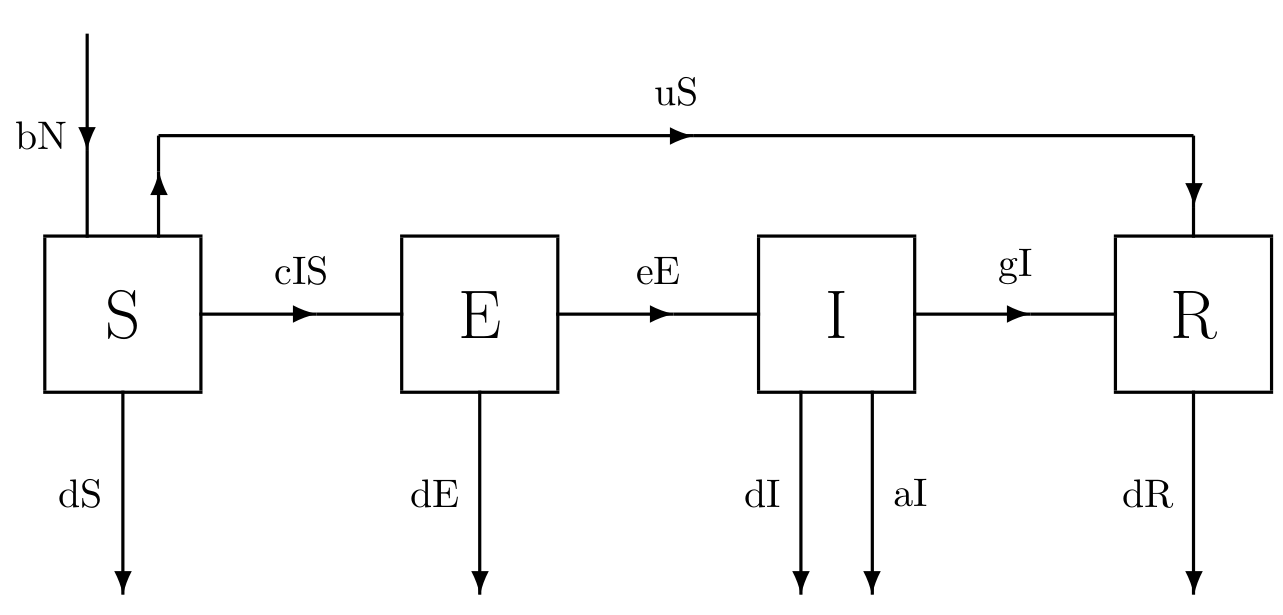
\includegraphics[width = \textwidth]{../images/flow-chat-seir.png}
        \caption{O gráfico de fluxo do modelo é explicado aqui.}
        \label{fig1:seir}
    \end{figure}

    \item Tratamento HIV
    
    Nesse laboratório é estudado a estratégia de tratamento por quimioterapia
    de inibidores da transcrição reversa para o HIV, considerando o sistema
    imunológico do indivíduo, em especial as células CD4+ T que são as mais
    afetadas no processo. A ideia desse controle é inibir a infecciosidade dos
    vírus livres em infectar células suscetíveis. 
    
    \item População de Ursos

    A população de ursos em um parque genérico com proximidade a áreas
    habitadas por humanos é considerada, de forma que essas regiões são
    compartilhadas, o que permite encontros indesejados entre ursos e humanos.
    A caça de ursos tanto na floresta quanto no parque são levados em
    consideração como forma de controle. 

    \item Modelo de Glucose 
    
    Alguns sistemas de equações diferenciais são sensíveis a mudanças nos
    parâmetros. Isso pode até levar a falta de convergência, dentre outros
    problemas. Neste laboratório, examinamos um problema mal condicionado. O
    modelo considerado tem o objetivo de melhorar a habilidade do teste GTT
    para detectar pré-diabetes e diabetes menos severas. especial considera a
    concentração de glucose no sangue e a concentração hormonal líquida. 
 
\end{enumerate}

\chapter{Linear Dependence on the Control}
\label{ch:17}
Vamos considerar problemas especiais em que o problema é linear 
no controle $u(t)$. 

\subsection{Controle Bang-Bang}

Considere o problema de controle ótimo.

$$max_u \int_{t_0}^{t_1} f_1(t,x) + u(t)f_2(t,x) dt$$
$$s.a.~~x'(t) = g_1(t,x) + u(t)g_2(t,x), x(0) = x_0$$
$$ a \leq u(t) \leq b$$

Assim $H(t,x,u,\la) = f_1(t,x) + \la g_1(t,x) + u(t)(f_2(t,x) + \la g_2(t,x))$, 
linear em $u(t)$. Observe a derivada parcial em relação a $u$ não
carrega informação sobre $u(t)$. Assim definimos $\psi(t) := f_2(t,x(t)) + \la(t)g_2(t,x(t))$,
muitas vezes chamada de função de troca. Se $\psi = 0$ não pode ser obtido 
em um intervalo de tempo, mas ocorre apenas em pontos finitos, o controle
é dito "Bing Bang", porque só varia entre os valores mínimo e máximo de $u(t)$. 
Os valores de $u(t)$ nesses pontos não são de interesse, portanto. 

Em contrapartida, se $\psi(t) \equiv 0$ em um intervalo de tempo, dizemos que $u^*$ é 
singular nesse intervalo. Esse caso será explorado na próxima sessão. 

Para resolver esse tipo de problema, primeiro precisamos verificar se de fato 
o problema é Bang-Bang. Numericamente, o problema é apenas em verificar a positividade
ou negatividade da função de troca. 

\subsection{Controles Singulares}

O livro explora um exemplo inicial:

$$max_u \int_0^2 (x(t) - t^2)^2 dt $$
$$s.a. ~~ x'(t) = u(t), x(0) = 1$$
$$0 \leq u(t) \leq 4$$

Calculamos o Hamiltoniano e encontramos $u^*(t)$ em função da adjunta. 
Para sair dessa hipótese, precisamos fazer uma análise mais minunciosa. 
Ela começa em provar que $x(t) \geq t^2 \rightarrow \lambda'(t) \leq 0 \wedge \la(t) \geq 0$. 
Então, basta encontrar os valores de $t$ em que essa função é positiva 
ou igual a $0$. Dessa forma, teremos descrito o controle e estado ótimos.

No caso numérico, podemos ter que analisar quando nossa função de troca vai ser 
maior, igual ou menor que zero. Porém, a igualdade a $0$ é complicada computacionalmente. 
Nesse sentido, estabelecemos um intervalo. No exemplo 17.4 do livro, quando o controle é 
Bang-Bang, houve convergência. Já o contrário não ocorreu. Como a função de troca é 
identicamente zero, problemas singulares são frequentemente instáveis. 

Pesquisa tem sido feita nesse sentido. A condição de Legendre-Clebsch é um exemplo. É uma
condição de segunda ordem, porque envolve ordem de derivadas mais altas.

\bibliography{book}


\end{document}